\documentclass[12pt]{article}
\usepackage{pgfplots, url, tikz, graphicx}
\usepackage{enumitem} % To customize enumerate
\usepackage{amssymb}
\usepackage{amsmath}
\usetikzlibrary{arrows.meta, positioning}
\pgfplotsset{compat=1.18}

\title{Math HW Week 1}
\author{Duc Nguyen}
\date{\today}

\begin{document}
\maketitle
\section*{Section 1.1}
\subsection*{\#1}
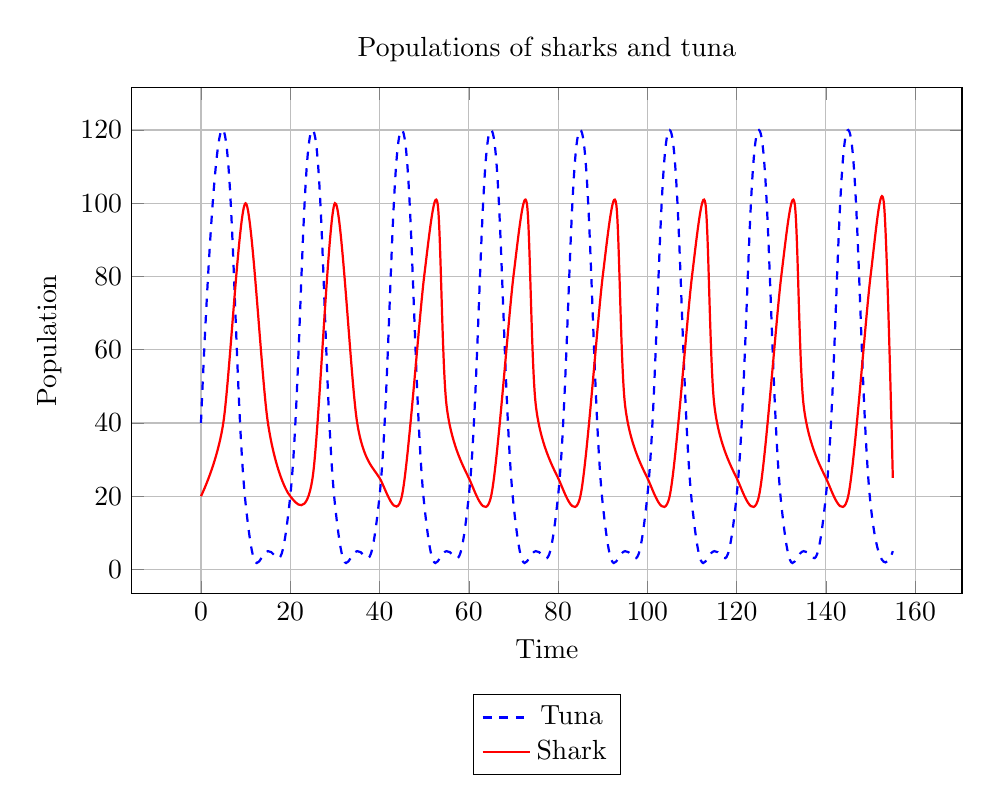
\begin{tikzpicture}
    \begin{axis}[
        title={Populations of sharks and tuna},
        xlabel={Time},
        ylabel={Population},
        legend style={at={(0.5,-0.20)}, anchor=north},
        grid=major,
        width=\textwidth,
        height=8cm
    ]
    \addplot[blue, thick, dashed, smooth, tension=0.8] coordinates {
        (0,40) (5,120) (10,18) (15,5) (20,20) (25,120) (30,18) (35,5)
        (40,20) (45,120) (50,18) (55,5) (60,20) (65,120) (70,18) (75,5) (80,20) (85,120)
        (90,18) (95,5) (100,20) (105,120) (110,18) (115,5) (120,20) (125,120) (130,18) (135,5)
        (140,20) (145,120) (150,18) (155,5) 
    };
    \addlegendentry{Tuna}
    
    \addplot[red, thick, smooth, tension=0.5] coordinates {
        (0,20) (5,40) (10,100) (15,40) (20,20) (25,25)
        (30,100) (35,40) (40,25) (45,20) (50,80) (53,100)
        (55,45) (60,25) (65,20) (70,80) (73,100)
        (75,45) (80,25) (85,20) (90,80) (93,100) (95,45)
        (100,25) (105,20) (110,80) (113,100) (115,45) (120,25)
        (125,20) (130,80) (133,100) (135,45) (140,25) (145,20)
        (150,80) (153,100) (155,25) 
    };
    \addlegendentry{Shark}
    \end{axis}
\end{tikzpicture}

I tried to sketch it as much similar as when I sketch it by hand.
However, due to some limitations of using Latex that I as a beginner can cover as much, 
the graph doesn't look exactly like the book but it should cover enough cycles

\subsection*{\#2}
Based on your Week 1 video:
\begin{center}
    \url{https://youtu.be/reG5KkAB3DY?si=SnSZelMbM2CZzi3A}
\end{center}
Positive feedback loop and negative feedback loop can be found on a similar situation about
loving someone and hating someone.
\begin{itemize}
    \item Positive feedback loop: 
    \begin{itemize}
        \item You're happy (+)
        \item I'm happy (+)
        \item You're sad (-)
        \item I'm sad (-)
    \end{itemize}
    \item Negative feedback loop:
    \begin{itemize}
        \item You're happy (+)
        \item I'm sad [because I hate you] (-)
        \item You're sad (-)
        \item I'm happy [because I hate you] (+)
    \end{itemize}
\end{itemize}

\subsection*{Further Exercise 1.1}
\begin{enumerate}
    \item a. Positive feedback loop, student studied, prepared more (+), got good grades (+),
    will get more confident and enjoyed the class (+), student did poorly (-), will put less effore (-),
    and get loweer grades (-)
    
    b. There're 2 major ways theoritically:
    
    \begin{itemize}
        \item Help my friends to study and prepare more, so they can get good grades (adding positive feedback)
        \item Stop them from putting less effort (removing negative feedback)
    \end{itemize}
\end{enumerate}

\section*{Section 1.2}
\subsection*{\#1}
A one-way water pipe, water can only go on one route (input), then through another pipe (output)

\noindent When you use your laptop to type a document, the words you type are input to the computer, and the document that appears on the screen is output from the computer.

\subsection*{\#2}
For a function to not be a function, it must have at least one input that has more than one output. So we can modify the menu to has multiple prices for one of the items or all of the items.

\subsection*{\#4}
$f(x) = x + 2$

\noindent $g(x) = x - 1$

\subsection*{\#7}
Because the Martian's RNA code has a 60\% chance of translated to serine, and 40\% chance of translated to histidine, it's not a function because there's no clear output for one RNA code.

\subsection*{\#8}
\begin{enumerate}[label=\alph*.]
    \item Total cost of Mocha $= 3.45 * 1.1 = 3.795$. Total cost of Latte $= 3.15 * 1.1 = 3.465$
    \item If the price of the drink is $x$, and the sales tax is a function of the drink times the tax rate, then
    \begin{equation}
        f(x) = (x * 1.1)
    \end{equation}
    where the total cost is represented by $f(x)$, and the tax rate is $1.1$ (10\% tax)
\end{enumerate}

\subsection*{Further Exercise 1.2}
\begin{enumerate}
    \item a. Price is a function of the item, because one item can only have one price (input with one output).

    b. Item is a function of the price because one item can only have one price (input with one output).
    
    c. One way is to make the entire menu cost the same price, so the price is not a function of the item.

    \item The vertical line test works because it's ensure that by crossing the graph with a vertical line, intersecting the graph at most once, that only one output is produced for each input, that input can't have multiple outputs although that's not always the case (*cough cough* polar coordinates *cough cough*)
    
    \item a. Spam $\rightarrow$ urco $\rightarrow$ 21 18 3 15

    b. Aisha's code went through a process called transcription, then through translation by implementing Tim's code, becomes an another output. Similar to the process of DNA transcription and translation.
    
    c. No, they can't. There's no set definition for numbers, so Tim's code can't be applied to Aisha's to encode a message. Likewise, codomains (inputs) can't be transcribed and translated back into domains (outputs).

    \item The domain for $\log(x)$ limits any number that less than or equal to 0, because the logarithm of a negative number is undefined. When you put in $\log(sinx)$, $sinx$ has to be bigger than 1, but $sinx$ itself has a domain of $[-1, 1]$, which can't satisfy the logarithm's domain. Therefore the function is not defined. To be specific, the codomains of a domains has to have limits or conditions that can be satisfied by the domain in order to be a function.
    
    \item Unless there's a part of DNA codons that help identify itself on the list of several different codons, it's not possible to find a function that takes amino acids to DNA codons. 
    
    \item Composing functions is more well-known as substitute a variable or a function into another function to create a new function. Addition and multiplication are combining variables or functions to create a new function. It's worth noting that although they might achieve the same purpose, they are in retrospect has a different approach to the problem.
\end{enumerate}

\section*{Section 1.3}
\subsection*{\#1}
\begin{enumerate}[label=\alph*.]
    \item Population density: subject per $(mi^2)$ or $(km^2)$
    \item Concentration of drugs:
    $(mmol/L)$ or $(nmol/L)$
    \item Amount of energy in an electrical appliance: ampere-hours $(Ah)$ or watt-hours $(Wh)$
\end{enumerate}

\subsection*{\#2}
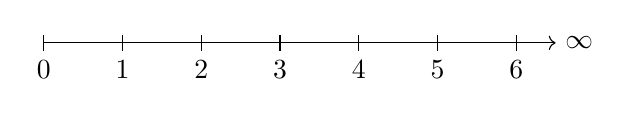
\begin{tikzpicture}
    % Draw number line from 0 to right (infinity symbolically)
    \draw[->] (0,0) -- (6.5,0) node[right] {$\infty$};
  
    % Tick marks and labels
    \foreach \x in {0,...,6}
      \draw (\x,0.1) -- (\x,-0.1) node[below] {\x};
\end{tikzpicture}

There can be many ants or infinite number of them, but can't be negative. So it's in the same vein as a population one-dimensional state space.

\subsection*{\#3}
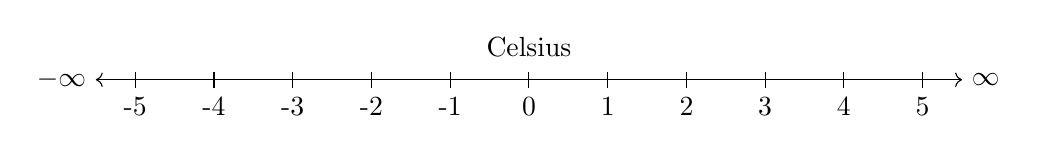
\begin{tikzpicture}
    % Draw the line
    \draw[<->] (-5.5,0) -- (5.5,0); 
    
    % Tick marks and labels
    \foreach \x in {-5,-4,...,5}
      \draw (\x,0.1) -- (\x,-0.1) node[below] {\x};

    \node[left] at (-5.5,0) {$-\infty$};
    \node[right] at (5.5,0) {$\infty$};
    \node[above=5pt] at (0,0) {Celsius};
  \end{tikzpicture}

The temperature can be anywhere from negative to positive, from a few degree in your house to a gigantic numbers of degree when checking the sun's interior, so it's in the same vein as an infinity one-dimensional state space.

\subsection*{\#4}
\begin{enumerate}[label=\alph*.]
    \item $5(10,2)$ = $[5*(10), 5*(2)]$ = $(50, 10)$
    \item $(4,7) + (3,9)$ = $(4+3, 7+9)$ = $(7, 16)$
    \item $2(3,2) - 3(5,4)$ = $(2*3 - 3*5, 2*2 - 3*4)$ = $(-9, -10)$ 
\end{enumerate}

\subsection*{\#5}
% Resize TikZ picture to fit textwidth
\resizebox{\textwidth}{!}{%
\begin{tikzpicture}
  \begin{axis}[
    width=\textwidth, % Set the width of the plot
    height=12cm, % Set the height of the plot
    axis lines = middle, % Draw axes in the middle
    xlabel = {Juveniles}, % Label for the x-axis
    ylabel = {Adults}, % Label for the y-axis
    xlabel shift = 10pt, % Shift the x-axis label 10pt to the right
    ylabel shift = 10pt, % Shift the y-axis label 10pt upwards
    xtick = {0, 50, 100, 150, 200}, % Tick marks on x-axis
    ytick = {0, 50, 100, 150, 200}, % Tick marks on y-axis
    grid = both, % Draw both major and minor grids
    grid style={line width=0.5pt, draw=gray!20}, % Grid style
    legend style={at={(0.5,-0.15)}, anchor=north, legend columns=-1, font=\footnotesize}, % Legend style
    title={\Large Black bear population}, % Title of the graph
    enlarge x limits={abs=1cm}, % Ensure there's some space on the x-axis
    enlarge y limits={abs=1cm}, % Ensure there's some space on the y-axis
    ]
    
    % Plot some points
    \addplot[only marks, red, mark size=3pt] coordinates {(200, 100)}; % Point 1
    \addplot[only marks, blue, mark size=3pt] coordinates {(30, 50)}; % Point 2
    \addplot[only marks, green, mark size=3pt] coordinates {(0, 25)}; % Point 3

    \node at (200, 100) [anchor=north east, font=\small] {$(200, 100)$}; % Label for Point 1
    \node at (30, 50) [anchor=south west, font=\small] {$(30, 50)$}; % Label for Point 2
    \node at (0, 25) [anchor=south west, font=\small] {$(0, 25)$}; % Label for Point 3

    % Legend for the points
    \legend{A, B, C}

  \end{axis}
\end{tikzpicture}%
}
\begin{enumerate}[label=\Alph*.]
    \item 200 juveniles and 100 adults
    \item 30 juveniles and 50 adults
    \item 0 juveniles and 25 adults
\end{enumerate}

\subsection*{\#6}
\resizebox{\textwidth}{!}{%
\begin{tikzpicture}
  \begin{axis}[
    width=\textwidth, % Set the width of the plot
    height=12cm, % Set the height of the plot
    axis lines = middle, % Draw axes in the middle
    xlabel = {Time}, % Label for the x-axis
    ylabel = {Population}, % Label for the y-axis
    xlabel shift = 10pt, % Shift the x-axis label 10pt to the right
    ylabel shift = 10pt, % Shift the y-axis label 10pt upwards
    xtick = {0, 50, 100, 150, 200}, % Tick marks on x-axis
    ytick = {0, 50, 100, 150, 200}, % Tick marks on y-axis
    grid = both, % Draw both major and minor grids
    grid style={line width=0.5pt, draw=gray!20}, % Grid style
    legend style={at={(0.5,-0.15)}, anchor=north, legend columns=-1, font=\footnotesize}, % Legend style
    title={\Large Populations of Sharks and Tunas}, % Title of the graph
    enlarge x limits={abs=1cm}, % Ensure there's some space on the x-axis
    enlarge y limits={abs=1cm}, % Ensure there's some space on the y-axis
    ]
    
    % Plot some points
    \addplot[only marks, blue, mark size=3pt] coordinates {(6, 80)}; % Point 1
    \addplot[only marks, red, mark size=3pt] coordinates {(20, 20)}; % Point 2
    \addplot[only marks, green, mark size=3pt] coordinates {(28, 80)}; % Point 3
    \addplot[only marks, black, mark size=3pt] coordinates {(42, 20)}; % Point 4
    \addplot[only marks, yellow, mark size=3pt] coordinates {(50, 80)}; % Point 5

    \node at (6, 80) [anchor=north west, font=\small] {$(6, 80)$}; % Label for Point 1
    \node at (20, 20) [anchor=south west, font=\small] {$(20, 20)$}; % Label for Point 2
    \node at (28, 80) [anchor=south west, font=\small] {$(28, 80)$}; % Label for Point 3
    \node at (42, 20) [anchor=north east, font=\small] {$(42, 20)$}; % Label for Point 1
    \node at (50, 80) [anchor=north east, font=\small] {$(50, 80)$}; % Label for Point 1

    % Legend for the points
    \legend{6 hours, 20 hours, 28 hours, 42 hours, 50 hours}

  \end{axis}
\end{tikzpicture}%
}
Based on the graph about population of sharks and tuna shown previously, where x represents the number of hours (times) past and y represents the population of sharks and tuna when both are equal to each other.

\subsection*{\#7}
\begin{tikzpicture}[scale=1]
    % Draw axes
    \draw[->] (-4,0) -- (4,0) node[right] {$x$};
    \draw[->] (0,-4) -- (0,4) node[above] {$y$};
  
    % Draw vector from origin to (3,2)
    \draw[->, thick, blue] (0,0) -- (3,2) node[above right] {$\vec{v}$};
    % Draw vector from origin to (-3,-2)
    \draw[->, thick, red] (0,0) -- (-3,-2) node[below left] {$-\vec{v}$};
  
    % Optional: label the coordinates
    \node[below right] at (3,2) {$(3,2)$};
    \node[above left] at (-3,-2) {$(-3,-2)$};
  \end{tikzpicture}

\subsection*{\#8}
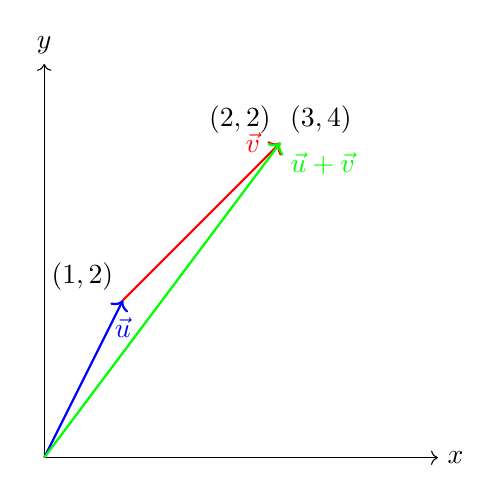
\begin{tikzpicture}[scale=1]
    % Draw axes
    \draw[->] (0,0) -- (5,0) node[right] {$x$};
    \draw[->] (0,0) -- (0,5) node[above] {$y$};
  
    % Draw vector from origin to (1,2)
    \draw[->, thick, blue] (0,0) -- (1,2) node[yshift=-10] {$\vec{u}$};
    % Draw vector from (1,2) to (2,2)
    \draw[->, thick, red] (1,2) -- (3,4) node[xshift=-10] {$\vec{v}$};
    % Draw vector from origin to (3,4)
    \draw[->, thick, green] (0,0) -- (3,4) node[below right] {$\vec{u} + \vec{v}$};
  
    % Optional: label the coordinates
    \node[above left] at (1,2) {$(1,2)$};
    \node[above left] at (3,4) {$(2,2)$};
    \node[above right] at (3,4) {$(3,4)$};
\end{tikzpicture}

$\vec{u} + \vec{v} = (1,2) + (2,2) = (3,4)$

\subsection*{\#9}
\begin{enumerate}[label=\alph*.]
    \item $(1,2,3) + (-2,0,5) = (1+(-2),2+0,3+5) = (-1,2,8)$
    \item $-3(4,6,-9) = (-3*4,-3*6,-3*-9) = (-12,-18,27)$
    \item $(2,4) + (1,3,5)$ = Undefined because both vectors don't have the same number of components (even though usually we can bypass this in calculus by implicitly adding 0 to the missing component)
    \item $5((0,1) + (7,3)) = 5(0,1) + 5(7,3) = (5*0,5*1) + (5*7,5*3) = (0,5) + (35,15) = (0+35,5+15) = (35,20)$
\end{enumerate}

\subsection*{\#10}
Usually, we would symbolize a 3-dimensional state space in real number notation as $\mathbb{R}^3$, for 18-dimensional state space we would use $\mathbb{R}^{18}$

\subsection*{Further Exercise 1.3}
\begin{enumerate}
    \item $\begin{bmatrix} 5 \\ 1 \end{bmatrix} - \begin{bmatrix} 3 \\ 2 \end{bmatrix} = \begin{bmatrix} 5 - 3 \\ 1 - 2 \end{bmatrix} = \begin{bmatrix} 2 \\ -1 \end{bmatrix}$
    \item \[
    \begin{aligned}
    (80, 400, 520) + (25, 130, 300)
    &= (80 + 25,\ 400 + 130,\ 520 + 300) \\
    &= (105,\ 530,\ 820)
    \end{aligned}
    \] 
    
    So the total would be 105 acres of meadows, 530 acres of pine forest, and 820 acres of broadleaf forest.
\end{enumerate}

\section*{Section 1.4}
\subsection*{\#1}
\begin{enumerate}[label=\alph*.]
    \item $A = 2.5B$
    \item $X = -3.7Z$
    \item $P = Bm$
\end{enumerate}

\subsection*{\#2}
\begin{enumerate}
    \item The amount of battery left in a cell phone
    \item The amount of gas in a car
    \item The amount of crops in a field
\end{enumerate}

\subsection*{\#3}
\begin{enumerate}
    \item The amount of battery left in a cell phone
    
    Inflow: Electrical charge
    Outflow: Phone activity (screen on, apps running)
    
    \item The amount of gas in a car

    Inflow: Gasoline from the gas station
    Outflow: Gasoline used by the car

    \item The amount of crops in a field
    
    Inflow: Water, fertilizer, sunlight
    Outflow: Harvested crops, evaporation
\end{enumerate}

\subsection*{\#4}
\begin{enumerate}
    \item 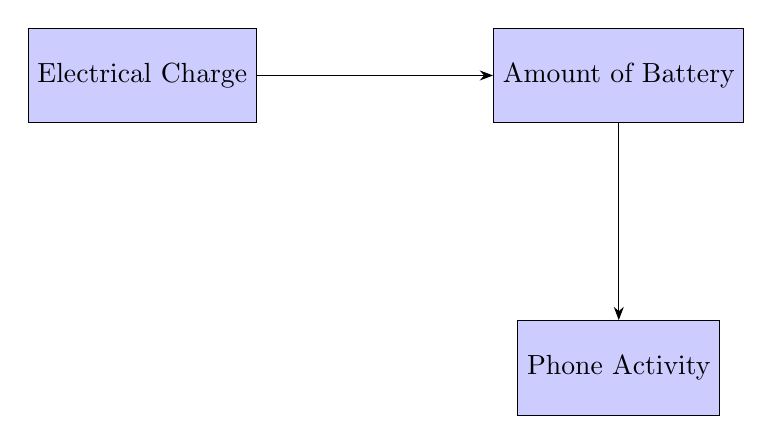
\begin{tikzpicture}[
        node distance=2.5cm and 3cm, % controls spacing between boxes
        every node/.style={draw, minimum width=2.5cm, minimum height=1.2cm, align=center},
        ->, % arrow style
        >=Stealth % arrowhead style
      ]
      
      % Nodes
      \node (A) [fill=blue!20] {Electrical Charge};
      \node (B) [fill=blue!20, right=of A] {Amount of Battery};
      \node (C) [fill=blue!20, below=of B] {Phone Activity};
      
      % Arrows
      \draw (A) -- (B);
      \draw (B) -- (C);
      
    \end{tikzpicture}
    \item 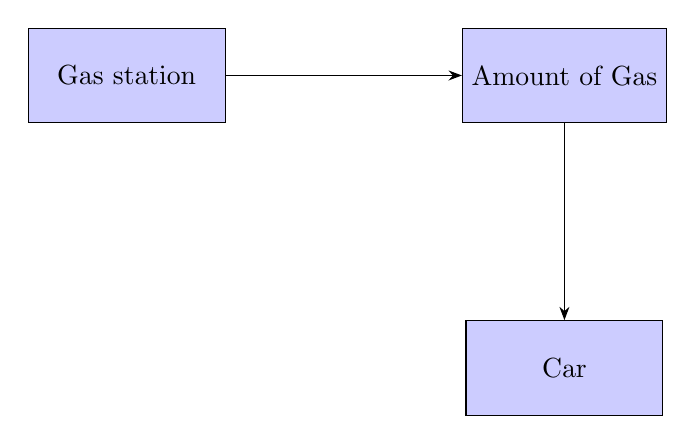
\begin{tikzpicture}[
        node distance=2.5cm and 3cm, % controls spacing between boxes
        every node/.style={draw, minimum width=2.5cm, minimum height=1.2cm, align=center},
        ->, % arrow style
        >=Stealth % arrowhead style
      ]
      
      % Nodes
      \node (A) [fill=blue!20] {Gas station};
      \node (B) [fill=blue!20, right=of A] {Amount of Gas};
      \node (C) [fill=blue!20, below=of B] {Car};
      
      % Arrows
      \draw (A) -- (B);
      \draw (B) -- (C);
      
    \end{tikzpicture}
    \item 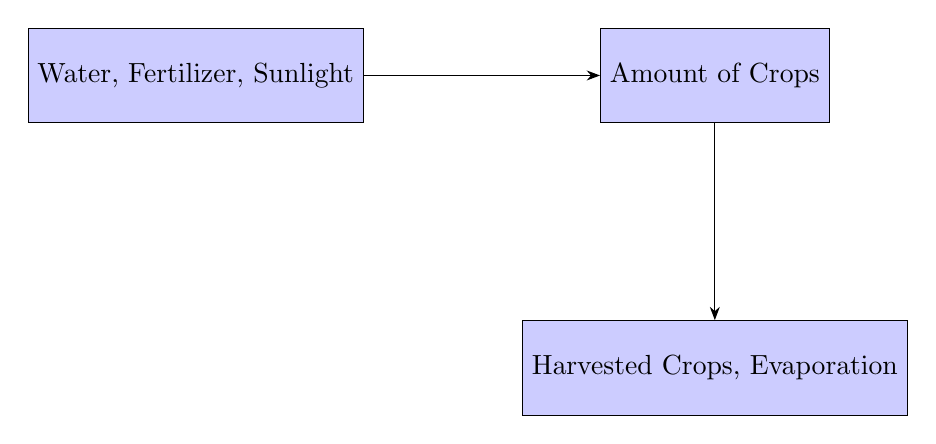
\begin{tikzpicture}[
        node distance=2.5cm and 3cm, % controls spacing between boxes
        every node/.style={draw, minimum width=2.5cm, minimum height=1.2cm, align=center},
        ->, % arrow style
        >=Stealth % arrowhead style
      ]
      
      % Nodes
      \node (A) [fill=blue!20] {Water, Fertilizer, Sunlight};
      \node (B) [fill=blue!20, right=of A] {Amount of Crops};
      \node (C) [fill=blue!20, below=of B] {Harvested Crops, Evaporation};
      
      % Arrows
      \draw (A) -- (B);
      \draw (B) -- (C);
      
    \end{tikzpicture}
\end{enumerate}

\subsection*{\#5}
\begin{enumerate}[label=\alph*.]
    \item change in the amount of battery = -energy used by the flashlight, \dots
    \item change in the amount of money in the bank account = $deposit + interest - withdrawal$
\end{enumerate}

\subsection*{\#6}
\begin{enumerate}
    \item Change in the amount of battery = $electrical charge - phone activity$
    \item Change in the amount of gas = $gas station - gasoline used by the car$
    \item Change in the amount of crops = $water + fertilizer + sunlight - harvested crops - evaporation$
\end{enumerate}

\subsection*{\#7}
Because there's only the outflow in the change equation, there's no inflow (The amount of tissue you use each week is 7, but you never/there's no way to refill it. So the change in the amount of tissue is negative, and the amount of tissue will decrease over time.)

\subsection*{\#8}
$L' = 1000$

\subsection*{\#9}
$P' = 100 + 3 - 95 - 2 = 6$

\subsection*{\#10}
\begin{enumerate}[label=\alph*.]
    \item $X' = 0.3x$
    \item $X' = -0.4x$
    \item $X' = 0.25x - 0.15x = 0.10x$
    \item $X' = 0.1x - 0.2x = -0.1x$
\end{enumerate}

\subsection*{\#11}
The population is growing in a and c, shrinking in b and d

\subsection*{\#12}
When X is larger than k, $X/k$ will become a number bigger than 1, which the right hand side of the equation will be negative, so the population will decrease.

\subsection*{\#13}
$R' = -kR - J$

Juliet doesn't change because Romeo's change doesn't affect her.

\subsection*{\#16}
$T' = bT - \beta ST$, where $b$ is the birth rate of the tuna, $\beta$ is the rate of any encounter which leads to sharks eat tuna, and $ST$ is the probability of find a sharks and tuna.

A deduction from this formula may occur that because the tuna is the prey, the more tuna there are, the more sharks will eat them, because tuna can't fight back and becomes a food source for sharks. So the population of tuna is mostly depends on the population of sharks, assume that every encounter between sharks and tuna will lead to a tuna being eaten.
\subsection*{\#17}
$B' = kA$ because A turns to B at rate $k$, so B absorbs A at rate $k$, means it's a positive equation.

\subsection*{\#18}
$B' = 2kA^2$ because 2 molecules of A combined to form each molecule of B

\subsection*{\#19}
B would be the same I think, because the rate of A is the same as the rate of B, for C I think it would be $C' = kAB$ because C is formed by A and B, so the rate of C is formed by combined A and B at rate $k$

\subsection*{\#20}
$B' = k_b C - k_f AB$

$C' = k_f AB$

\subsection*{Further Exercise 1.4}
\begin{enumerate}
    \item \begin{enumerate}[label=\alph*.]
        \item $B' = 100$
        \item $P' = -5$
        \item $H' = 0.02H$
        \item $G' = -0.07G$
        \item $L' = 0.05L + 0.09L = 0.14L$
        \item $K' = 4K - 3K = K$
        \item $P' = 2.5P + 10 - 1.3P - 0.6P = 0.6P + 10$
    \end{enumerate}
    \item \begin{enumerate}[label=\alph*.]
        \item For 1 or each individual, it would be $1/k$
        \item For $X$ individuals, it would be $X/k$
        \item The fraction of resources not being used is $1 - X/k$
        \item $X'/X = 1 - r X/k$
        \item $X' = X(1 - r X/k)$
    \end{enumerate}
    \item $L' = 0.1L - 0.4 - 0.02L = 0.08L - 0.4$
    \item $P' = f - dP - kP^3$
    \item $M' = r(m - M) -fM^2 -dM$
    \item Let $V$ be the vole population, $O$ is the owl population:
    
    $V' = 0.075V - 0.01VO$

    $W' = 0.0005VO - 0.1O$
    \item Let $H$ be the horse population, $W$ is the wolf population:
    
    $H' = 0.15H - 0.01H^2 - 0.02HW$

    $W' = 0.05W$
    \item Let $K$ be the Kelp population, $U$ is the Urchin population, $S$ is the Sea Otter population:
    
    $K' = 0.02K - 0.01K^2 - 0.05KU$
    
    $U' = 0.01KU - 0.01U - 0.03US$
    
    $S' = 0.0003US - 0.001S$
    \item Let $W$ for the number of people that's walking around, $F$ for the number of people that's riding ferris wheel, $C$ is the number of people that's eating ice cream:
    
    $W' = E - dW - bW^2 - mW/C + n(1-z)F + kC$

    $F' = bW^2 - nF$

    $C' = mW/C + znF - kC$
    \item \begin{enumerate}[label=\alph*.]
        \item $U'$ has a positive term $vW$ and death terms $-mU$ and $-pU$, $V'$ has a birth/growth like term and loss terms $-mV$ and $-rVW$ suggesting infection worsens when meeting with susceptible individuals, $W'$ is created by $rVW$ and lost by $-mW$ and $-vW$, which leads to U being susceptible by conclusions (since $vW$ create $U$), $V$ is infected but not showing symptoms and $W$ is being symptomatic
        \item \begin{enumerate}[label=\roman*.]
            \item Reduce the infection coefficient $r$ to a smaller value 
            \item Reduce $r$ more or introduce a delay to transition somehow
            \item Add a new variable in $V'$, specifically add a positive term to $U'$ and a matching negative term to $V'$
        \end{enumerate}
    \end{enumerate}
\end{enumerate}
\end{document}